\documentclass[a4paper,11pt,liststotocnumbered,bibtotocnumbered]{scrartcl}
\usepackage[french]{babel}
\usepackage[utf8]{inputenc}
\usepackage[T1]{fontenc}
\usepackage{pst-all}
\usepackage{vanadin}
\usepackage{isotope}
\usepackage{longtable}
\usepackage{color}
\usepackage{amsmath}
\usepackage{units}
\usepackage{float}


\subject{TP~5 Physique nucléaire}
\title{Etude du flux du rayonnement cosmique}
\subtitle{Rayonnement cosmique}
\author{Mona Dentler, Sabine Engelhardt}
\publishers{Université Joseph Fourier, Grenoble}
\date{\today}

\begin{document}
 \nocite{poly}
 \pagestyle{empty}
 \begin{center}
  \makeatletter
   %\titlefont
  \@subject
  \vspace{2cm}

  \Huge
  Etude du flux du rayonnement cosmique\newline
  \vspace{1cm}
  \Large


  \@author
  \newline
  \@publishers


  \@date
  \makeatother
 \end{center}
 \vfill

 \begin{abstract}
  Le rayonnement cosmique qui bombarde en permanence l'atmosphère terrestre, consiste des particules de très haute énergie de l'origine solare, galactique ou intergalactique. Ces particules interagissent avec les particules de l'atmosphère et créent des particules secondaires de durée plus ou moins court. Au niveau de sol on peut détecter pour la plupart des muons.\\
  Dans cette TP nous mesurons le flux de muons crées par le rayon cosmique à l'aide de trois détecteurs de particules chargées. Ceux-ci sont monté une sur l'autre avec un certain distance pour permettre une mesure de co\"{\i}ncidence entre les détecteurs. Pour obtenir un bon résultat il faut premièrement calibré le système à l'aide des mesures préliminaires et deuxièment il faut calcule l'efficacité des détecteurs et les défauts peut-être par bruit mesuré.
 \end{abstract}
\newpage
 \pagestyle{scrheadings}
 \tableofcontents
\newpage

 \begin{section}{Théorie}
   \todo{Sabine: übersetzen und kürzen, ev. Antworten ergänzen}
   Luftschauer entstehen, wenn die primäre kosmische Strahlung aus dem Weltall auf die Erdatmosphäre trifft. Von dem hochenergetischen primären Teilchen oder Photon werden über eine Kaskade eine Vielzahl von Sekundärteilchen erzeugt. Die primäre Kosmische Strahlung setzt sich wie folgt zusammen:
   \begin{figure}[htb]
    \centering
    \begin{tabular}{lcr}
     Wasserstoffkerne (Protonen) & $\simeq$ & 85~\%\\
     Heliumkerne ($\alpha$-Teilchen) & $\simeq$ & 12~\%\\
     Kerne mit Z $\geq 3$	& $\simeq$ & 2~\%\\ 
     Elektronen, $\gamma$-Strahlen	& $\simeq$ & 1~\%\\
    \end{tabular}\cite[S. 14]{burak}
   \end{figure}	

   Als Quellen für $\gamma$-Strahlung kommen nach \cite{astroteilchen} verschiedenste galaktische und extra-galaktische Objekte in Frage oder sind als solche identifiziert:
   \begin{itemize}
    \item Überreste von Sternexplosionen
    \begin{itemize}
     \item Neutronensterne
     \item Umfeld von schwarzen Löchern
    \end{itemize}
    \item Molekülwolken
    \item Starburst Galaxien
    \item Galaxienhaufen
    \item Aktive Galaxienkerne (AGNs)
    \item Gamma-Ray Bursts
   \end{itemize}
   Anhand der verschiedenen Komponenten der Sekundärstrahlung in einem Schauer können bei der Detektion am Erdboden Rückschlüsse auf die Primärstrahlung gezogen werden.
   Die Schauer von $\gamma$-Strahlung unterscheiden sich dabei sehr von denen, die durch Hadronen ausgelöst werden. Da das Ziel verfolgt wird, ein einfaches $\gamma$-Teleskop zu realisieren, ist es notwendig, die Unterschiede zwischen elektromagnetischen und hadronischen Kaskaden zu kennen.


   \subsection{Elektromagnetischer Schauer}
    Photonen können drei für die Entstehung von Sekundärteilchen relevante Arten von Wechselwirkung eingehen:
    \begin{enumerate}
     \item{Photoeffekt}
     \item{Compton-Effekt}
     \item{Elektron-Positron-Paarerzeugung}
    \end{enumerate}
    Während bei niedrigen Photon-Energien nur der Photoeffekt und Comptoneffekt möglich sind, kann, wenn die Photonenergie größer als die doppelte Ruheenergie des Elektrons ist, im elektrischen Feld eines Atomkerns ein Elektron-Positron-Paar erzeugt werden.

    Betrachtet man die Massenabsorptionskoeffizienten der einzelnen Effekte in Abhängigkeit der Photonenenergie (vgl. Abb.~\ref{fig:absorption}), wird klar, dass bei hochenergetischen $\gamma$-Quanten nur noch die Elektron-Positron-Paarerzeugung von Bedeutung ist.

    Durch Paarbildung entstehen ein Elektron und ein Positron und beide senden durch Bremsstrahlung sekundäre Photonen aus.

    Bei einer exakten Energiebilanz für den Paarbildungseffekt muss der meist vernachlässigte Rückstoß auf den Atomkerns der Masse $M$ mit einberechnet werden. Für die minimale Energie des $\gamma$-Quants ergibt sich:
    \begin{equation*}
     E_{\gamma, \idx{min}} = 2 m_{\idx{e}} c^2 \left( 1 + \frac{m_{\idx{e}}}{M} \right)
    \end{equation*}
    Paarbildung kann nicht im leeren Raum stattfinden, da dort Impuls und Energie nicht gleichzeitig erhalten bleiben können.\footnote{
    Dies wird an folgendem Beispiel klar:\\
    Man nehme an, ein Photon mit einer Energie von $ \hbar \omega $ zerfällt in ein Elektron und ein Positron mit je 	einer kinetischen Energie von $ (\gamma - 1)m_{\text{e}}c^2 $. Die einfachste Möglichkeit, wenn man versuchen will Energie und Impuls zu erhalten, wäre wenn sich das erzeugte Paar parallel zur Ausbreitungsrichtung des ursprünglichen Photons bewegt.\\
    \begin{tabular}{rl}
     Dann ist mit Energieerhaltung: & Energie d. Photons $= \hbar \omega = 2\gamma m_{\idx{e}}c^2$\\
     & Impuls des Paars $ = 2 \gamma m_{\idx{e}} v = (\hbar \omega / c)(v/c)$\\
     Aber: & Anfangsimpuls des Photons $ = \hbar \omega / c $
    \end{tabular}\\
    Da $v$ echt kleiner als $c$ sein muss, können Impuls- und Energieerhaltung im Vakuum also nicht simultan erfüllt sein.}
    Daher können $\gamma$-Photonen den Weltraum durchqueren und bilden erst in der Erdatmosphäre einen Schauer.

   \begin{figurehere}
    \center 
    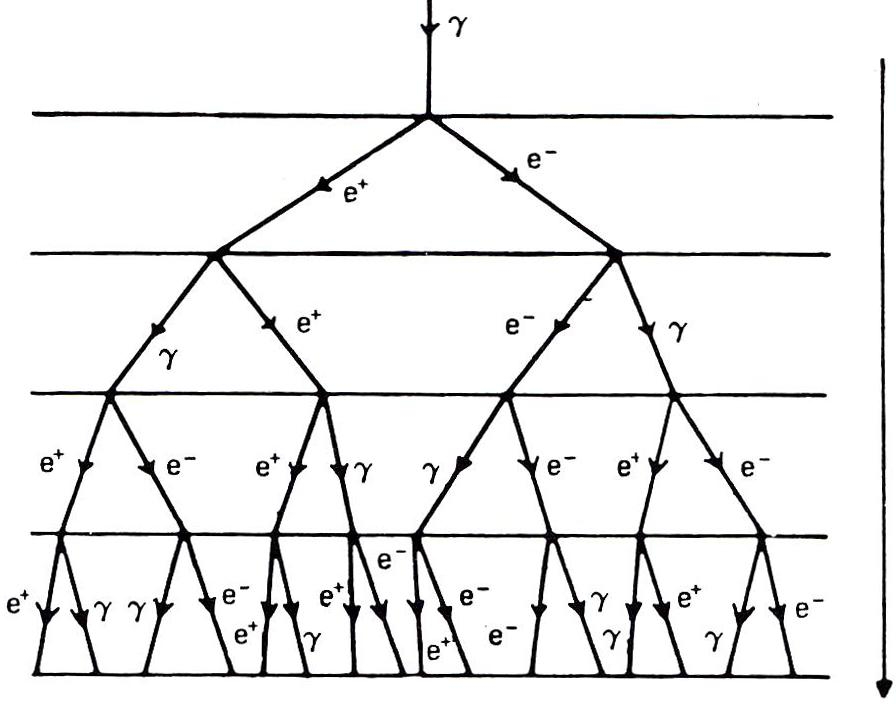
\includegraphics[width=0.5\textwidth]{bilder/emschauer.jpg}   
    \caption{Ablauf eines elektromagnetischen Schauers}   
    \label{fig:emschauer}   
   \end{figurehere}
     
  Abbildung \ref{fig:emschauer} zeigt ein einfaches Modell für einen elektromagnetischen Schauer, der durch $\gamma$-Strahlung erzeugt wird. 
  Das sekundäre Photon kann dann wiederum ein Elektron-Positron-Paar erzeugen. Die Kaskade hört auf, wenn die jeweilige Energie der Teilchen die Paarbildungsenergie unterschreitet und die Bremsstrahlung keine weiteren Photonen mehr erzeugen kann, die ihrerseits energiereich genug für die Paarbildung  sind.

 
  \subsection{Hadronische Kaskade}
   Hochenergetische Protonen oder schwerere Kerne, also die Hadronen der kosmischen Höhenstrahlung, stoßen in der Atmosphäre mit den Atomkernen der Luftmoleküle zusammen. Da im Mittel 50\% der hochenergetischen Protonen in der Atmosphäre bei einer Tiefe von ca. \unit[800]{kg\,m^{-2}} absorbiert werden und weil die Atmosphäre eine Tiefe von ca. $\unit[10\,000]{kg\,m^{-2}}$ ist \cite[S.~133]{longair} besitzt, reagieren die Teilchen bereits in den obersten Schichten und dringen nicht selbst bis zur Erdoberfläche durch. Nachgewiesen werden können sie daher nur über die von ihnen ausgelösten Sekundärteilchen-Schauer.

   Bei der Kollision entstehen vor allem $\pi^+$, $\pi^-$ und $\pi^0$, alle drei Sorten von Pionen.\footnote{Weitere Produkte können \emph{Strange Particles}, und selten auch (Anti-)Nukleonen sein.} Von der Wechselwirkung mit den Atomkernen sind meist nur eines bis zwei der Nukleonen im Target-Kern betroffen. Diese werden jedoch so stark beeinflusst, dass sie aus dem Atomkern herausgeschleudert werden.

   Nach einer hilfreichen empirischen Faustregel entstehen für einfallende Protonen mit einer Energie über \unit[1]{GeV} bei Kollisionen mit Luftmolekülen grob $2E^{1/4}$ neue, geladene und hochenergetische Teilchen, wobei $E$ in \unit{GeV} angegeben wird. Zur Veranschaulichung soll Abbildung  \ref{fig:preaktion} dienen.
   \begin{figure}[htb]
    \center
    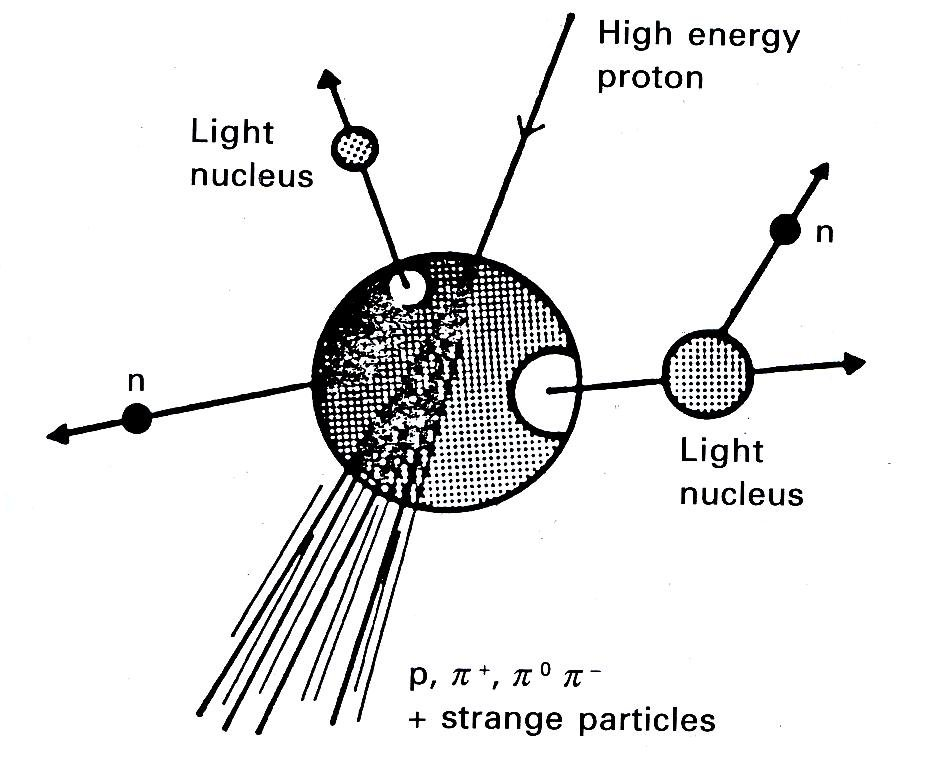
\includegraphics[width=0.6\textwidth]{bilder/03.jpg}
    \caption{Schematische Reaktion eines hochenergetischen Protons mit einem Atomkern in der Atmosphäre}
    \cite[S.~133]{longair}
    \label{fig:preaktion}
   \end{figure}

   Im Flug zerfallen viele der geladenen Pionen in Myonen über die Reaktionen
   \begin{equation*}
	\left.
	\begin{array}[]{lll}
		\pi^{+} & \rightarrow & \mu^{+} + \nu_{\mu}\\
		\pi^{-} & \rightarrow & \mu^{-} + \overline{\nu}_{\mu}\\	
	\end{array}
	\right\} \idx{mittlere Lebensdauer: } \unit[2,551\cdot10^{-8}]{s}
	\left.
	\begin{array}[]{lll}
	\pi^{0} & \rightarrow & 2\gamma	
	\end{array}
	\right\} \idx{mittlere Lebensdauer: } \unit[8,4\cdot10^{-17}]{s}
	\end{equation*}

   Die Myonen werden durch Ionisation abgebremst und zerfallen in Positronen, Elektronen und Myon- bzw. Elektron-(Anti-)Neutrinos

  \begin{equation*}
	\left.
	\begin{array}[]{lll}
		\mu^{+} & \rightarrow & \text{e}^{+} + \nu_{\text{e}} + \overline{\nu}_{\mu}\\
		\mu^{-} & \rightarrow & \text{e}^{-} + \overline{\nu}_{\text{e}} + \nu_{\mu}
	\end{array}
	\right\} \text{mittlere Lebensdauer: } \unit[2,2001\cdot10^{-6}]{s}
   \end{equation*}

   In den obersten Luftschichten entstehen viele der Myonen, bevor die Pionen Gelegenheit zu weiteren Kernwechselwirkungen haben. Die entstandenen Produkte fliegen in einer gewölbten Scheibe zum Erdboden. Die Wölbung rührt daher, dass die Teilchen mit einem größeren Streuwinkel einen etwas längeren Weg zum Erdboden zurücklegen müssen. Von der gewaltigen Anzahl an Sekundärteilchen erreichen nur noch die relativ langlebigen Myonen die Erdoberfläche und können dort detektiert werden. 

   \begin{figure}[htb]
    \center
    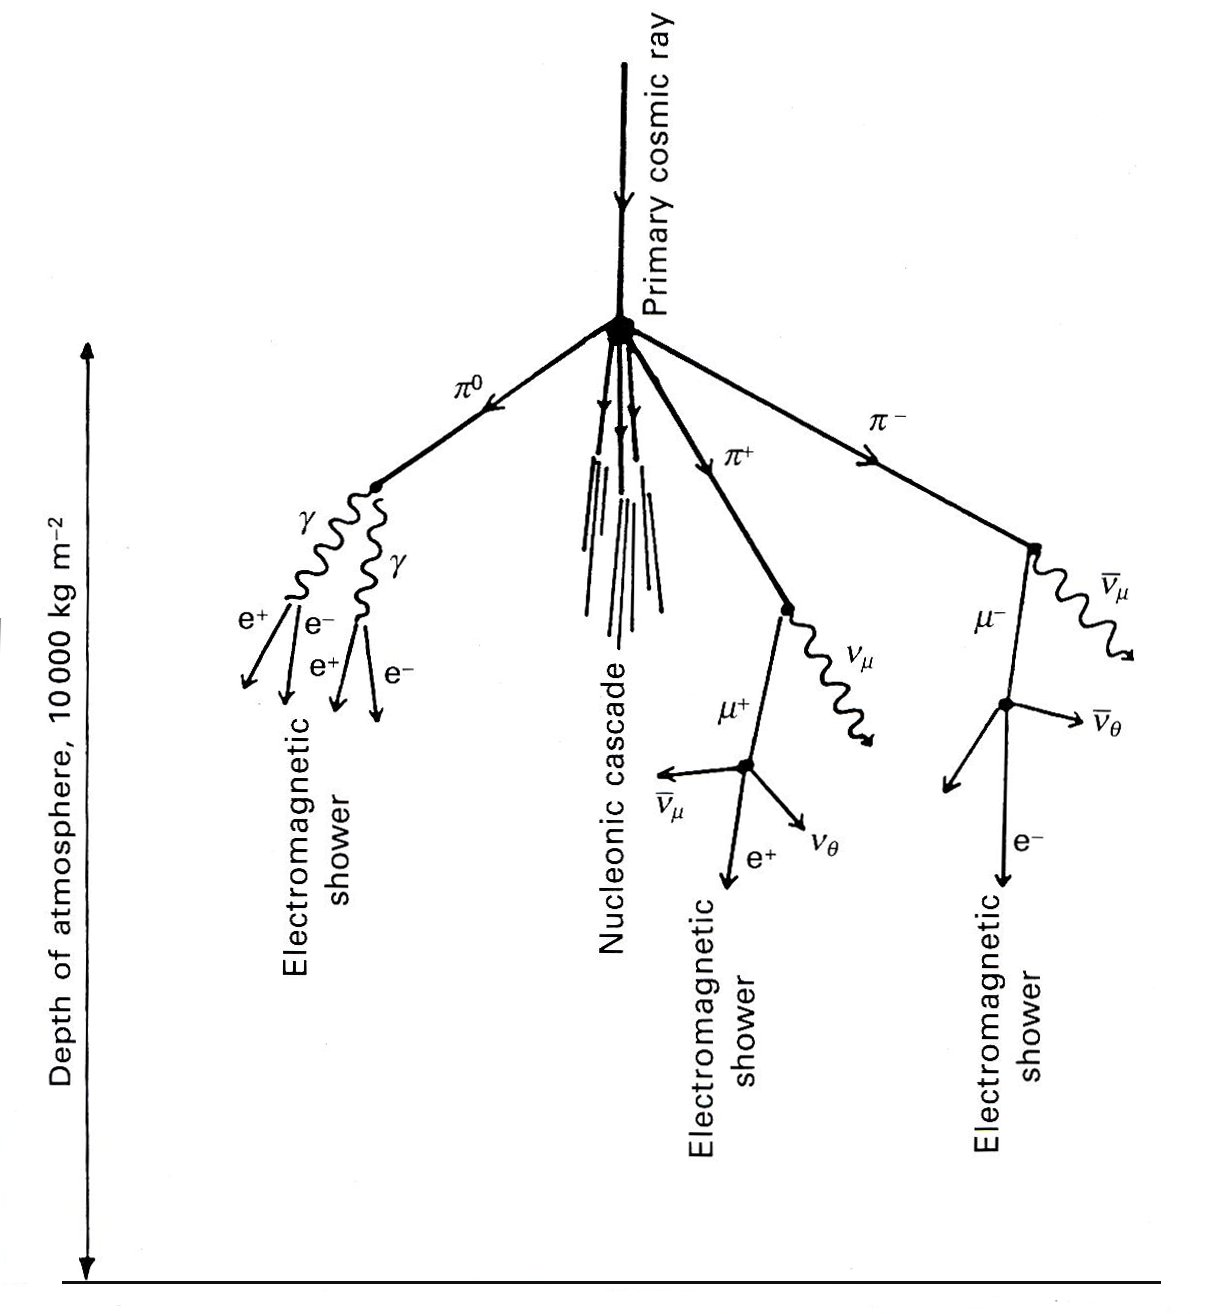
\includegraphics[width=0.7\textwidth]{bilder/hadronischer_schauer.jpg}
    \caption{Hadronischer Schauer}
   \end{figure}
 \end{section}
  
 \begin{section}{Préliminaire}
  \subsection{Préparation des photomultiplicateurs}
   \todo{ausführen}
   Pour obtenir une bonne mesure les signaux emettés des deux photomultiplicateurs doivent être précise. L'image suivant montre un bon signal d'un PMT en mesurant un photon $\gamma$. Il n' y a qu'un signal bien défini et à peine de bruit qui peut déranger le signal. Quand même il faut mettre un seuil (thresh) pour qu'on ne mesure que les vraies signaux.  
   \begin{center}
    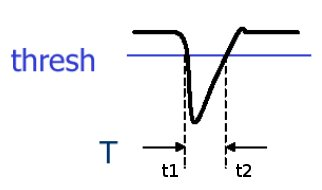
\includegraphics[width=0.5\textwidth]{bilder/pmtpuls.jpg}
   \end{center}
  

  \subsection{Réglage de la co\"{\i}ncidence}
   \todo{neue Daten einsetzen}
   \subsubsection{Générer un signal logique}
    Le module de co\"{\i}ncidences ne peut qu'évaluer des signaux logique, alors il faut générer un signal logique du signal analytique des PMT. Nous avons utilisé deux discriminateurs pour réussir à le faire. De fa\c con à pas obtenir des cascades des signaux à partir d'un seul signal, il faut ensuite mettre le seuil découvrit et mettre la largeur des créneaux à environ \unit[600]{ns}. Les signaux des deux PMT sont observés à l'oscilloscope aous l'aspect s'ils sont en co\"{\i}ncidence.
   
  
   \subsubsection{Comptage}
    Après avoir observer les signaux en co\"{\i}ncidence sur l'écran de l'oscilloscope (malheuresement nous n'avons pas réussi à faire un screenshot) nous avons relié les sorties des deux discriminateurs à un module de co\"{\i}ncidence. Le sortie de celui est connecté à l'echelle de comptage. Une mesure de \unit[10]{s} a montré que les signaux sont comptés.
   
   
   \subsubsection{Première mesure}
    \todo{Daten}
   

   \subsubsection{Interprétation} 
    Nous suposse que les dates sont decrit par la distribution de Poisson:
    \begin{equation*}
     P_{\mu}(n)=\frac{\mu^n}{n!}\cdot e^{-{\mu}}
    \end{equation*}
    Avec la moyenne $\mu$ et le nombre de fois $n$. On trouve pour $lim \; n {\rightarrow}  \infty$ que $\bar{n}$, la moyenne experimentale tend vers $\mu$ et l'écart type $\sigma$ vers $\sqrt{\mu}$:
    \begin{equation*}
     \bar{n}=\sum_{n=0}^{\infty} n \cdot P_{\mu}(n)=e^{-{\mu}}\sum_{n=1}^{\infty}\frac{\mu^n}{(n-1)!}=\mu \cdot  e^{-{\mu}}\sum_{k=0}^{\infty}\frac{\mu^k}{(k)!}=\mu \cdot e^{-{\mu}}\cdot  e^{{\mu}}=\mu
    \end{equation*}

    \begin{equation*}
     \begin{split}
      \sigma^2=\overline{(n-\bar{n}\,)^2}=\overline{n(n-1)}+\bar{n}-{\bar{n}}^2=\sum_{n=0} ^{N} n (n-1)\cdot P_{\mu}(n)+\mu -\mu^2=\\
      e^{-{\mu}}\sum_{n=2}^{\infty}\frac{\mu^n}{(n-2)!}+\mu -\mu^2=\mu^2+ \mu -\mu^2=\mu
     \end{split}
    \end{equation*}
    L'écart type de nos dates est dans les limites de $\sqrt{\mu}$ ce qui dit que les nombres mesurés sont bien. Il y a des petites différences qui peut être expliqué par le fait que plus des désintégration ou plus de bruit étaient mesuré.
   
  

  \subsection{Mesure en co\"{\i}ncidence}
   \todo{alles einsetzen}
   \subsubsection{Détection}
 

   \subsubsection{Bruit}
 \end{section}


 \begin{section}{Mesure}
  
 \end{section}


 \begin{section}{Conclusion}
  
 \end{section}
 
 \begin{appendix}
  \bibliographystyle{unsrt}
  \bibliography{literatur}  

  \listoffigures  
 \end{appendix}

\end{document}

